\documentclass{EESD}
% To change the slides size go to EESD.cls file and edit the preamble as explained.

% Important packages to be called
\usepackage{subcaption} % for adding sub-figures
\usepackage{graphicx}
\usepackage[T1]{fontenc}
\usepackage{tikz} % for cool graphics and drawings
\usepackage{listings}
\usepackage{syntax}
\usepackage[absolute,overlay]{textpos} % To place the figures by coordinates (x,y) - Beamer doesn't support floats XD
\usepackage{multicol} % To adjust items and stuff automatically in a number of a pre-specified columns
\graphicspath{{Figures/}}
\usepackage[utf8]{inputenc}
\usepackage{amsmath}
\usepackage{amsfonts}
\usepackage{amssymb}
\usepackage{hyperref}
% fonts packages
\usepackage{ragged2e} % Justified typesetting

\setbeameroption{hide notes} % Only slides
% \setbeameroption{show only notes} % Only notes
% \setbeameroption{show notes on second screen=right} % Both

% For adding code blocks
\usepackage{listings}
\definecolor{keywordcolor}{rgb}{0.7, 0.1, 0.1}   % red
\definecolor{tacticcolor}{rgb}{0.0, 0.1, 0.6}    % blue
\definecolor{commentcolor}{rgb}{0.4, 0.4, 0.4}   % grey
\definecolor{symbolcolor}{rgb}{0.0, 0.1, 0.6}    % blue
\definecolor{sortcolor}{rgb}{0.1, 0.5, 0.1}      % green
\definecolor{attributecolor}{rgb}{0.7, 0.1, 0.1} % red
\def\lstlanguagefiles{lstlean.tex}
\lstdefinelanguage{Toy}{
  keywords={free, let, if, while},
  ndkeywords={true, false},
  sensitive=false,
  comment=[l]{\#},
  basicstyle=\tt\scriptsize,
  keywordstyle=\color{blue}\bfseries,
  ndkeywordstyle=\color{magenta}\bfseries,
  identifierstyle=\color{black},
  commentstyle=\color{darkgray},
  rulecolor=\color{black},
}

\lstset{
    language=Toy,
    breaklines=true,
    numbers=left,
    numberstyle=\tiny\color{black},
    escapechar=@,
    frame = single,
}

\author{
	Guillem Bartrina I Moreno \and
	Franco Sainas \and
	Marcin Wojnarowski
}
\title[Formal properties of a toy language]{Formally verifying properties of a toy language}

\institute[ENAC]{{\'Ecole Polytechnique F\'ed\'erale de Lausanne (EPFL)}{\newline\newline CS550 - Formal Verification}}
\subject{Course project}
\date{December 2023}

\begin{document}
{
\usebackgroundtemplate{}
\coverpage{
    \titlepage{~}
    % To add additional text to the title components
}
}

\setbeamertemplate{logo}{} % To override the logo from the other slides and delete it completely


% -----------------------Table of contents TOC Three Styles
% Explicitly split the TOC if it's too long
% \begin{frame}[allowframebreaks]{Outlines}
% \tableofcontents[sections={1-3}] % Explicitly split TOC
% \framebreak
% \tableofcontents[sections={4-7}] % Explicitly split TOC
% \end{frame}

% % Just a normal TOC 
% \begin{frame}[allowframebreaks]{Outlines}
% \tableofcontents
% \end{frame}

% Use smart division for the TOC
\begin{frame}{Outline}
    \begin{multicols}{2}
        \tableofcontents
    \end{multicols}
\end{frame}

% -----------------------Introduction
\section{Introduction}

\begin{frame}{Introduction}
    \begin{itemize}
        \item Vast majority of programming languages do not have a formally verified core \note[item]{Leads to memory errors, unsoundness, and general unsafety}
        \item Functional languages are studied a lot, but the real world is messy and dominated by imperative languages
        \item The goal is to define a toy language for which we can formally reason about some properties\note[item]{Toy meaning created for studying purposes rather than real world applications.}
    \end{itemize}
\end{frame}


% -----------------------Toy language
\section{Language}
\breakingframe{Language}

\subsection{Description}
\begin{frame}{Description}
    \begin{itemize}
        \item Imperative \note[item]{Functional languages have been studied a lot, imperative languages dominate the market}
        \item The only value type is a \textbf{boolean} \note[item]{We are not studying types but memory}
        \item All variables are "heap" allocated
        \item Lexical scoping
        \item Started ambitious (product types, references, deep mutability)\pause, \textit{quickly} humbled
    \end{itemize}
\end{frame}

\subsection{Syntax}

\begin{frame}[fragile]{Syntax}

    \begin{columns}
        \begin{column}{0.4\textwidth}
            \begin{lstlisting}
let myVar = true
let other = false

if other @$\uparrow$@ other {
    myVar := myVar @$\uparrow$@ other
    free other
}

while myVar {
    let p = myVar @$\uparrow$@ true
    myVar := p @$\uparrow$@ (p @$\uparrow$@ p)
}
\end{lstlisting}
        \end{column}

        \begin{column}{0.6\textwidth}
            \setlength{\grammarindent}{6em}

            % manually aligning labels...
            \begin{grammar}
                <expr> ::= true | false \qquad\;\;\;\; \texttt{Bool}
                \alt <expr>$_1$ $\uparrow$ <expr>$_2$ \; \texttt{Nand}
                \alt <name> \qquad\qquad\;\, \texttt{Ident}
                \alt (<expr>) \qquad\qquad\: \texttt{Group}

                <stmt> ::= let <name> = <expr> \quad\;\;\,\texttt{Decl}
                \alt <name> := <expr> \qquad\;\, \texttt{Assign}
                \alt if <expr> \{ <stmt> \} \quad\;\; \texttt{If}
                \alt while <expr> \{ <stmt> \} \ \texttt{While}
                \alt free <name> \qquad\qquad\quad\, \texttt{Free}
                \alt <stmt>$_1$ <stmt>$_2$ \qquad\quad\; \texttt{Seq}
            \end{grammar}
        \end{column}
    \end{columns}

\end{frame}


\subsection{Semantics}

\begin{frame}[fragile]
    \frametitle{Semantics}
    \begin{itemize}
        \item $\texttt{Free}$ conservatively forbids further usage of the variable
              \begin{lstlisting}[gobble=12, numbers=none, basicstyle=\linespread{0.89}\tt\scriptsize]
            let var = true
            if false {
                free var
            }
            var = false # illegal
        \end{lstlisting}
        \item $\texttt{Decl}$ defines a variable in its scope
              \begin{lstlisting}[gobble=12, numbers=none, basicstyle=\linespread{0.89}\tt\scriptsize]
            if false {
                let var = true
            }
            var = false # not accessible
        \end{lstlisting}
        \item $\texttt{Decl}$ cannot shadow
              \begin{lstlisting}[gobble=12, numbers=none, basicstyle=\linespread{0.89}\tt\scriptsize]
            let var = true
            if false {
                let var = true # illegal
            }
        \end{lstlisting}
    \end{itemize}
\end{frame}


% -----------------------Approach
\section{Approach}

\breakingframe{Approach}

% Approach:
%   - Proving them on paper is not exactly what we did in the course
%   - A program can be seen as a complex tree-like structure (AST)
%   - Decided to implement an interpreter of the language, which is essentially a computer program that operates over the said structure and outputs results.
%   - Given that the input structure has some properties, equivalent to a (type) checker, we prove that out tree-walk interpreter program has some properties (invariants)

\begin{frame}{Approach}

    \begin{block}{}
        Implement an interpreter for our toy language. Given that a program is valid, prove that its execution by the interpreter enjoys some properties.
    \end{block}

    %Our approach to proving properties about the toy language we have defined is
    %Implement interpreter + prove properties of that interpreter
    %\textit{Interpreter can be viewed as complex program that operates over complex data structure which is the abstract syntax tree of the program.}
    %If the input program has some properties, guaranteed by checker, then the execution of the interpreter on that program enjoys some properties (no throw).

    \vspace{0.2cm}

    \begin{center}
        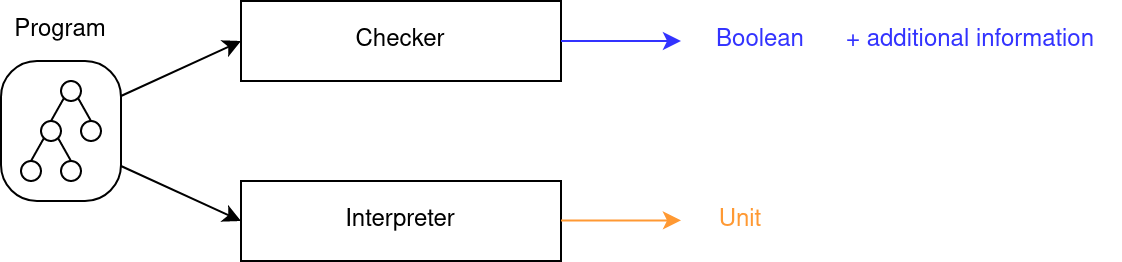
\includegraphics[height = 0.4\textheight]{Figures/approach.png}
    \end{center}

    \vspace{0.2cm}

    \textbf{Goal:} \  \textcolor{blue}{Program is valid} \ $\Rightarrow$ \  \textcolor{orange}{Program executes successfully (does not throw)}

\end{frame}

% -----------------------Abstract machine
\subsection{Abstract state machine}

\begin{frame}{Abstract state machine}
    \begin{tabular}{rl}
        Environment & \(env: \text{Name} \to \text{Abstract location}\)  \\
        Memory      & \(mem: \text{Abstract location} \to \text{Value}\) \\
        Allocator   & \(alloc: \_ \to \text{Abstract location}\)         \\
    \end{tabular}\\
    \vspace{0.5cm}
    \textbf{Abstract state:} \((env, mem, alloc)\)
\end{frame}

% -----------------------Properties

\section{Properties}

\breakingframe{Properties}

\subsection{Closedness}
\begin{frame}[fragile]{Closedness}

    All variable accesses exist in the current environment.

    \begin{definition}[Closedness]
        A program is closed if whenever evaluating $\texttt{Ident}\langle \text{name} \rangle$ or $\texttt{Assign}\langle \text{name}, \text{expr} \rangle$, $env(\text{name})$ is defined.
    \end{definition}

    \begin{lstlisting}
var1 := true # error
if var2 { # error
}
\end{lstlisting}
\end{frame}

\subsection{No redeclarations}
\begin{frame}[fragile]{No redeclarations}

    A declaration cannot declare an already declared name.

    \begin{definition}[No redeclarations]
        A program has no redeclarations if whenever evaluating $\texttt{Decl}\langle \text{name}, \text{expr} \rangle$, $env(\text{name})$ is not defined.
    \end{definition}

    \begin{lstlisting}
let var = true
let var = false # error
if true {
    let var = false # error
}
\end{lstlisting}
\end{frame}

\subsection{Unique ownership}
\begin{frame}{Unique ownership}

    No two variables in the environment point to the same location.

    \begin{definition}[Unique ownership]
        A program exhibits unique ownership when $env$ is injective at all times.
    \end{definition}
    \note[item]{This cannot actually happen in code, but this property is needed to ensure \texttt{Free} doesn't create dangling pointers.}
\end{frame}

\subsection{No use-after-free}
\begin{frame}[fragile]{No use-after-free}

    All variable accesses point to existing memory. \note[item]{Or more generally, no dangling pointers.}

    \begin{definition}[No use-after-free]
        A program has no uses-after-free if whenever evaluating $\texttt{Ident}\langle \text{name} \rangle$ or $\texttt{Assign}\langle \text{name}, \text{expr} \rangle$, $mem(env(\text{name}))$ is defined.
    \end{definition}

    \begin{lstlisting}
let var = true
free var
var := true # error
\end{lstlisting}
\end{frame}

% -----------------------Implementation

% 3 paths we started: small-step, big-step, lean
%   - Why 3, which is the one we advocate most for, what are the differences (advantages, disadvantages of each one)
%   - what we achieved so far (of what is prensented in the first to sections)

\section{Implementation}

\breakingframe{Implementation}

\begin{frame}{Implementation}
    \begin{itemize}
        \item Stainless interpreter (big-step flavour)
              \vspace{0.2cm}
        \item \textcolor{purple}{Lean interpreter}
              \vspace{0.2cm}
        \item \textbf{Stainless tracer (small-step flavour)}
    \end{itemize}

    % Lack of experience + lack of references -> not a clear direction to follow from the beginning. => Due to a number factors

    %We ended up implementing three versions of the interpreter and tried to prove the properties for each of them.
    % Initially, implemented big-step interpreter in Stainless and Lean, with the intention to empirically find out which of the two was most suitable for the project
    % We made similar progress with bot, but then got stuck with stainless and become afraid we would not be able to prove some things about whiles (cause termination). We decided to implement small-step interptreter in Stainless, which gives more precise control over the execution and we think would allow us to prove more interesting properties. => A bit later decided to implement small-step interpreter or tracer with hope of gainig more precie control over execution and being able to prove more properties in an inductive fashion.
    % [just random thoughts]

    \vspace{1cm}
    \noindent\hrulefill
    \vspace{0.5cm}

    Implementation details:
    \begin{itemize}
        \item Avoid throwing in Stainless: interpretation functions return either a set of exceptions or the actual result.   % EXPLANATION OF HOW WE DO HANDLE EXCEPTIONS WITH EITHER SET PROBLEM!!
        \item Limited interoperability between Maps and Sets in Stainless: introduce several axioms. % Comment about data structures
    \end{itemize}

\end{frame}

\subsection{Stainless interpreter}
\begin{frame}[fragile]{Stainless interpreter}

    % Most straightforward interpreter: interprets node and all children (if any) and returns state.

    % Actual scala signature?
    % Any code snippet?

    % List of proven properties? And auxiliar properties? Property dependency DG?
    % Program is closed
    % Auxiliar proof: variables in the environment are consistent with variables 

    \(Interpreter: Prog \to State\)

    Given a program \(Prog\), the interpreter returns the final state \(State\).

    \vspace{1cm}

    {\textbf{def evalStmt(stmt: Stmt, state: State): Either[Set[LangException], State]}}

    \vspace{1cm}

    \begin{itemize}
        \item Pros: Most natural design, straightforward implementation, \textit{closer} to the checker
        \item Cons: Symmetries with checker and proofs
    \end{itemize}

\end{frame}

\subsection{Stainless tracer}
\begin{frame}{Stainless tracer}
    %It is the model in which we have made the most progress, we should emphasize it! And describe what we have achieved and what it has cost.
    % Had to introduce _Block

    Interpreter problem with whiles: non termination. \\ \note[item]{Whiles introduce non terminating programs, which translates in a non terminating interpreter. At this point we thought it would be easier to reason about just one step of interpretation. For these reasons we decided to build a tracer.}

    \pause

    Given a program \(P\) the tracer returns a list of states.\\
    We mainly focus on the part of the tracer that given a program \(P\) and a state \(S\) returns the program \(P'\) the state \(S'\) given by one step of execution.
    \\
    \centering \(T: \text{Prog} \to \text{State}^*\)
    \\
    \centering \(T_1: \text{Prog} \times \text{State} \to \text{Prog} \times \text{State}\)
    \\

    \pause

    \note[item]{When interpreting a while, the tracer will evaulate the condition, and if it's true it will return a sequence of the body and the while loop.}

    \begin{itemize}
        \item Pros: More control over intermediate states, interesting properties about the trace.
        \item Cons: Many preconditions about the input state, prove preservation of properties. \note[item]{In the interpreter you don't have this problem.}
    \end{itemize}


    % Proving things using evidence from the checkes is way harder because of the very different paradigm.

    % Proven: closedness, no redeclarations
    % + preservation of closedness in one step
\end{frame}

\logo{\centering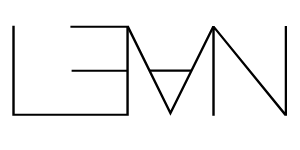
\includegraphics[height=1.43cm]{Figures/logo-lean.png}\vspace{220pt}}
\subsection{Lean interpreter}
\begin{frame}[fragile]{Lean interpreter}

    \begin{lstlisting}[language=lean]
partial def evalStmt
    (stmt : Stmt) (env : Env) (mem : Memory)
    (h : isTypeCheckedStmt stmt (keySet env))
    : Env × Memory := match stmt with
  -- ...
  | Stmt.conditional condition body =>
    let cond := evalExpr condition env mem (typeCheck_conditionalCond h)
    let (newEnv, newMem) := if cond
        then evalStmt body env mem (typeCheckStmt_conditionalBody h)
        else (env, mem)

    -- we drop the new env, but keep the new mem
    (env, newMem)
  -- ...
\end{lstlisting}

\end{frame}
\setbeamertemplate{logo}{}

% -----------------------Conclusions
\section{Conclusions}

\breakingframe{Conclusions}

\begin{frame}{Discussion}
    \begin{itemize}
        \item Performance has to be traded for provable correctness \note[item]{When defining something in a more performant way, it seemed to be often harder to prove its correctness}
        \item Symmetricity between properties and implementation \note[item]{Eases proofs that one implies the other}
        \item Requires intermediate lemmas proving correlation between properties and implementation \note[item]{The constructed env set in properties have to be related to the constructed env set in the interpreter}
        \item Proving correctness is hard and very time consuming
        \item Despite the language being a subset of our original design, we are happy with the results
    \end{itemize}
\end{frame}

\begin{frame}{Future work}
    \begin{itemize}
        \item Lack of memory leaks \note[item]{Not a memory safety property per-se, it conflicts with the definition of no use-after-free}
        \item More language features \note[item]{Requires careful design to understand how they interact with other existing features}
    \end{itemize}
\end{frame}

\breakingframe{Merci!}


\end{document}
